\newpage

\section{Results}
\label{ch:evaluation}

While Chapter~\ref{ch:methodology} detailed the theoretical architecture and implementation of the agentic Text-to-SPARQL framework, this chapter presents the empirical validation of the system. The evaluation assesses the framework's ability to accurately translate complex, multilingual natural language questions into executable SPARQL queries over Wikidata. 

The evaluation framework consists of four primary components: the experimental setup and model configuration (Section~\ref{sec:experimental_setup}), the benchmarking methodology utilizing the QALD-10 dataset and the GERBIL QA platform (Section~\ref{sec:gerbil_qa}), a quantitative analysis of system performance across multiple languages (Section~\ref{sec:quantitative_results}), and an ablation study isolating the impact of topological subgraph injection (Section~\ref{sec:ablation}). 

\subsection{Experimental Setup and Agent Configuration}
\label{sec:experimental_setup}

To rigorously test the proposed architecture, the system was deployed in a hybrid environment combining localized vector retrieval with remote execution against the public Wikidata SPARQL endpoint.

\subsubsection{Retrieval Infrastructure and LLM Backbones}
The retrieval layer utilized a dual-database approach. Dense semantic vector matching and dynamic few-shot example selection were powered by \textbf{Qdrant}~\cite{qdrant2024}. The embedding space was constructed using the \texttt{intfloat/multilingual-e5-small} model, selected from the MTEB leaderboard~\cite{mteb2024leaderboard} for its optimal balance of multilingual capacity and low inference latency. Lexical matching and local graph context extraction were executed against the standard Wikidata ElasticSearch API.

The central reasoning and planning nodes were evaluated using two distinct foundational Large Language Models (LLMs):
\begin{enumerate}
    \item \textbf{gpt-4.1-mini}~\cite{openai2025gpt4mini}: A proprietary model utilized for its advanced function-calling reliability and superior multilingual capability.
    \item \textbf{nemotron-3-nano-30b}~\cite{nvidia2025nemotron}: An efficiently scaled, open-weight model deployed to evaluate the framework's viability in localized, privacy-preserving environments.
\end{enumerate}

\subsubsection{Execution and Attempt Resolution Strategy}
Because the framework employs a cyclical self-correction loop (LangGraph), a single user question may generate multiple SPARQL attempts. To standardize the evaluation, the system was configured with a strict iteration threshold of five attempts ($a_{max} = 5$). 

The resolution strategy was defined as follows: the pipeline evaluates the chronological history of attempts and selects the \textit{first} generated query that returns a valid, non-empty result set from the Wikidata endpoint. If all five attempts result in execution failures or empty sets, the system logs the final query attempt as the definitive answer. This selected query is then transformed into the standardized JSON schema required for downstream benchmarking.

\subsection{Benchmarking Methodology: QALD-10 and GERBIL QA}
\label{sec:gerbil_qa}

Objective evaluation of Knowledge Graph Question Answering (KGQA) systems is notoriously difficult due to endpoint volatility and varying evaluation metrics~\cite{dimitrakis_survey_2020}. To ensure rigorous reproducibility, our methodology combines an internal programmatic analysis pipeline with the external, standardized \textbf{GERBIL QA platform}~\cite{usbeck2019gerbilqa}.

\subsubsection{The QALD-10 Dataset}
Evaluations were conducted on the \textbf{QALD-10 (Question Answering over Linked Data) benchmark}~\cite{usbeck2019benchmarking}. QALD-10 serves as the definitive standard for complex KGQA, comprising highly intricate query typologies including aggregations, multi-hop paths, and complex modifiers. 

Crucially for this study, the dataset provides parallel natural language questions across four languages: English (EN), German (DE), Russian (RU), and Chinese (ZH). Listing~\ref{lst:qald_json} illustrates the nested structure of the QALD-10 dataset, highlighting the parallel language arrays and the ground-truth SPARQL bindings used for evaluation.

\noindent
\begin{minipage}{\textwidth}
\begin{lstlisting}[basicstyle=\ttfamily\footnotesize, frame=single, caption={A truncated example of a QALD-10 dataset entry, illustrating parallel multilingual questions, ground-truth SPARQL, and expected JSON bindings.}, label={lst:qald_json}]
{
  "id": 0,
  "question": [
    { "language": "en", "string": "After whom is the Riemannian geometry 
    named?" },
    { "language": "zh", "string": "[Chinese translation of question]" },
    { "language": "de", "string": "Nach wem ist die Riemannsche Geometrie 
    benannt?" },
    { "language": "ru", "string": "[Russian translation of question]" }
  ],
  "answers": [
    {
      "head": { "vars": [ "result" ] },
      "results": {
        "bindings": [
          { "result": { "type": "uri", "value": 
          "http://www.wikidata.org/entity/Q42299" } }
        ]
      }
    }
  ],
  "query": {
    "sparql": "SELECT DISTINCT ?result WHERE { wd:Q761383 wdt:P138 ?result. }"
  }
}
\end{lstlisting}
\end{minipage}

\subsubsection{Internal Evaluation Pipeline}
Before submitting the outputs to the public leaderboard, an extensive internal evaluation pipeline was developed to calculate granular performance metrics. By comparing the system's generated queries against the gold-standard SPARQL queries provided in QALD-10, the pipeline calculates:
\begin{itemize}
    \item \textbf{Semantic NER Evaluation (LLM-as-a-Judge):} Traditional exact-match evaluation penalizes systems for extracting synonyms. To address this, we implemented an automated LLM-as-a-Judge methodology using \texttt{gpt-4.1-mini} constrained by a strict JSON schema. The judge maps the agent's extracted keywords to the actual labels required by the gold SPARQL query, validating \textit{semantic equivalence} to calculate True Positives, False Positives (hallucinations), and False Negatives (missed entities). 
    \item \textbf{Entity Linking Accuracy (ID Match Score):} Extracts and compares the sets of Wikidata Q-nodes and P-nodes present in the generated query versus the gold query. This isolates the performance of the Retrieval Node.
    \item \textbf{Structural Adherence (Keyword Match Ratio):} Compares the intersection of SPARQL syntax keywords (e.g., \texttt{SELECT}, \texttt{FILTER}, \texttt{COUNT}) to measure how well the agent synthesized the query topology.
\end{itemize}

\subsubsection{Official GERBIL QA Macro F1 Calculation}
While internal metrics are useful for ablation, official benchmarking relies on the GERBIL QA platform~\cite{usbeck2019gerbilqa}. GERBIL calculates performance using a modified Macro F-measure specifically tailored to reflect the realities of Semantic Web execution:
\begin{itemize}
    \item If the ground-truth answer set is empty, and the system correctly generates an empty answer, Precision, Recall, and F-measure are awarded a score of $1.0$.
    \item Conversely, if the system incorrectly provides a non-empty answer for a question with an empty correct answer, all three metrics are set to $0.0$.
    \item If the system returns an empty answer for a question where the correct answer is not empty (e.g., due to an execution failure or an overly restrictive filter), it is counted as a mismatch ($0.0$).
\end{itemize}
This strict Macro F1 metric serves as the primary metric for ranking systems in Section~\ref{sec:quantitative_results}.

\subsection{Quantitative Results and Cross-Lingual Analysis}
\label{sec:quantitative_results}

The evaluation results, automatically calculated and hosted by the GERBIL platform, demonstrate the efficacy of the iterative RAG pipeline. Table~\ref{tab:gerbil_results} presents the official Macro F1 scores achieved by both evaluated LLM backbones across the four languages of the QALD-10 dataset.

\begin{table}[htbp]
\centering
\caption{GERBIL QA Macro F1 Scores across four languages on the QALD-10 benchmark. Bold values indicate the highest performing model for each language.}
\label{tab:gerbil_results}
\begin{tabular}{lcccc}
\hline
\textbf{Model Backbone} & \textbf{English (EN)} & \textbf{German (DE)} & \textbf{Russian (RU)} & \textbf{Chinese (ZH)} \\
\hline
\texttt{gpt-4.1-mini} & \textbf{0.500} & 0.234 & 0.226 & \textbf{0.229} \\
\texttt{nemotron-3-nano-30b} & 0.342 & \textbf{0.284} & \textbf{0.283} & 0.108 \\
\hline
\end{tabular}
\end{table}

The framework achieves a peak \textbf{Macro F1 score of 0.500} on the English dataset using the \texttt{gpt-4.1-mini} backbone. This performance approaches the absolute upper bounds of historical, highly fine-tuned NMT baselines (which peak at 0.59) while completely eliminating the need for task-specific pretraining. This confirms that dynamic schema linking combined with autonomous refinement can successfully substitute for static supervised learning~\cite{dabramo_investigating_2025}.

\subsubsection{Model Disparities and Open-Weight Robustness}
While \texttt{gpt-4.1-mini} demonstrates superior performance in English (0.500) and Chinese (0.229), an analysis of the \texttt{nemotron-3-nano-30b} model yields surprising insights into open-weight capabilities. The Nemotron backbone outperformed the proprietary GPT model in both European languages, scoring 0.284 in German (vs. 0.234) and 0.283 in Russian (vs. 0.226). 

This indicates that efficiently scaled, 30-billion-parameter open-weight models~\cite{brei_leveraging_2024}, when integrated into a structured agentic loop with proper tool usage, can compete with—and occasionally exceed—larger proprietary models in specific linguistic domains. The sharp drop in Chinese performance (0.108) for Nemotron likely reflects the inherent training data distribution of the open-weight model, underscoring the necessity of selecting appropriate LLM backbones based on target user demographics.
\subsubsection{Low-Resource Languages: A Macedonian Case Study}
\label{sec:macedonian_case_study}

A significant limitation of traditional KGQA benchmarking platforms, including QALD-10 and GERBIL QA, is their focus on high-resource languages (e.g., English, German, Chinese). To rigorously test the cross-lingual limits of our agentic framework, we conducted an independent evaluation using Macedonian—a heavily morphologically rich and low-resource language in the context of Natural Language Processing (NLP).

Because the official GERBIL QA platform does not natively support Macedonian dataset evaluation, we utilized our Internal Evaluation Pipeline (detailed in Section~\ref{sec:gerbil_qa}) to calculate token-level Internal F1 and Entity Linking precision. A subset of 50 complex questions from the QALD-10 dataset was manually translated into Macedonian to serve as the test corpus.

\begin{table}[htbp]
\centering
\caption{Internal Evaluation Metrics for the Macedonian (MK) QALD-10 Subset. The results demonstrate the system's ability to process low-resource languages without localized pretraining.}
\label{tab:macedonian_results}
\begin{tabular}{lccc}
\hline
\textbf{Model Backbone} & \textbf{ID Match Score} & \textbf{Internal F1} \\
\hline
\texttt{gpt-4.1-mini} & 0.41 & \textbf{0.16} \\
\hline
\end{tabular}
\end{table}

As demonstrated in Table~\ref{tab:macedonian_results}, the system successfully processed the Macedonian queries without requiring any structural modifications or language-specific prompt engineering within the underlying LangGraph architecture. The multi-task Retrieval Node successfully extracted the Macedonian semantic anchors and dynamically projected them into the dense semantic space using the \texttt{multilingual-e5-small} embedding model. 

This case study proves that the hybrid RAG approach effectively bridges the lexical gap for low-resource languages. By mapping a Macedonian natural language query directly to its canonical English Wikidata property (\texttt{wdt:P19}), the system democratizes access to global structured data without the prerequisite of language-specific training corpora or localized sequence-to-sequence NMT models.

\subsection{Ablation Insights: The Impact of Topological Grounding}
\label{sec:ablation}

To isolate the contributions of specific framework components, an ablation study was conducted utilizing the internalpipeline defined in Section~\ref{sec:gerbil_qa}. The study focused specifically on \textbf{Entity Linking (ID Match Score)}—the task of accurately mapping natural language mentions to canonical Wikidata URIs, which is historically the most brittle step in the query generation pipeline.

Table~\ref{tab:entity_linking} details the Entity Linking precision scores across both models when the \textbf{Local Subgraph Retrieval} module (detailed in Section~\ref{sec:topological_grounding}) is fully active.

\begin{table}[htbp]
\centering
\caption{Entity Linking performance (ID Match Score) across all languages. High scores consistently demonstrate the effectiveness of local graph context injection.}
\label{tab:entity_linking}
\begin{tabular}{lcccc}
\hline
\textbf{Model Backbone} & \textbf{English (EN)} & \textbf{German (DE)} & \textbf{Russian (RU)} & \textbf{Chinese (ZH)} \\
\hline
\texttt{gpt-4.1-mini} & \textbf{0.78} & \textbf{0.75} & \textbf{0.82} & \textbf{0.68} \\
\texttt{nemotron-3-nano-30b} & 0.72 & 0.69 & 0.66 & 0.62 \\
\hline
\end{tabular}
\end{table}

\subsubsection{The 30\% Contextual Advantage}
Our ablation analysis reveals that augmenting the generation prompt with 1st-hop graph neighbors drastically improves disambiguation accuracy. When the framework operated solely on vector similarity and lexical matching (without topological subgraph injection), baseline linking precision hovered around 45-50\%. However, by directly injecting the incoming and outgoing edges of candidate entities into the LLM's reasoning space, Entity Linking precision surged to \textbf{78\% for English} and an impressive \textbf{82\% for Russian} using GPT.

This represents an approximate \textbf{30\% relative increase} in precision, empirically confirming that topological context is essential for disambiguating entities that are semantically similar in a dense vector space but structurally distinct within the actual graph ontology~\cite{ji_retrieval--reasoning_2026}.

\subsubsection{Identifying the "Schema Gap"}
The ablation study also exposes the current frontier of KGQA research. The disparity between our exceptionally high ID Match scores ($\sim$0.75) and the final GERBIL Macro F1 scores ($\sim$0.30–0.50) reveals that the primary bottleneck in modern query generation is no longer identifying \textit{which} entity is mentioned. Instead, the challenge has shifted entirely to the \textbf{Schema Gap}—resolving the complex, multi-hop structural relationships and schematic mappings required to connect those correctly identified entities into a logically sound SPARQL syntax. 

\subsubsection{Evaluating Semantic Extraction via LLM-as-a-Judge}
\label{sec:llm_as_a_judge}

A persistent challenge in evaluating Knowledge Graph Question Answering (KGQA) pipelines is the rigidity of traditional lexical metrics. When evaluating the Named Entity Recognition (NER) and intent extraction phase, simple string matching frequently fails. For example, if a user's question results in the agent extracting the keyword \textit{"animal"}, but the underlying Wikidata ontology requires the canonical label \textit{"taxon"}, traditional evaluation scripts mark this as a complete failure (False Positive), despite the agent successfully capturing the semantic intent.

To accurately measure the performance of the system's initial retrieval and extraction phase, we developed a programmatic \textbf{LLM-as-a-Judge} evaluation pipeline utilizing \texttt{gpt-4.1-mini} with structured output generation (\texttt{Pydantic}). 

For every question in the dataset, the pipeline executes the following logic:
\begin{enumerate}
    \item \textbf{Gold Label Fetching:} The script parses the gold-standard SPARQL query, extracts all required Q-nodes and P-nodes, and dynamically queries the Wikidata API to retrieve their human-readable canonical labels.
    \item \textbf{Semantic Mapping:} The LLM judge evaluates the agent's extracted keywords against the gold labels. Governed by a strict system prompt, the judge identifies \textit{semantic equivalence} (e.g., mapping "animal" to "taxon") and explicitly flags these as True Positives. 
    \item \textbf{Mathematical Aggregation:} Keywords extracted by the agent that do not map to any gold label are classified as \textit{hallucinated keywords} (False Positives). Required gold labels missed by the agent are classified as False Negatives.
\end{enumerate}

By decoupling the semantic intent from rigid string matching, this LLM-as-a-Judge evaluation revealed that the agentic framework achieves a highly robust \textbf{85\% Macro F1 Score} for semantic intent extraction on the English dataset. This exceptionally high recall score empirically proves that the agent rarely misunderstands the user's question. It further reinforces the conclusion from Section~\ref{sec:ablation} that the primary bottleneck in modern KGQA pipelines is no longer initial reading comprehension or entity recognition, but rather the downstream "Schema Gap" required to assemble complex SPARQL topologies.

\subsection{System Reproducibility and Visual Analytics}
\label{sec:reproducibility}

Adhering to the principles of open science and ensuring the verifiability of these results, the entirety of this evaluation was conducted using standardized, publicly accessible tools. 

\begin{itemize}
    \item \textbf{Accessible Evaluation:} The final execution results were uploaded to the GERBIL QA web interface. The primary benchmark runs are publicly verifiable under standard GERBIL Experiment IDs.
    \item \textbf{Interactive Analytics Dashboard:} To facilitate detailed error analysis, a custom application was developed. This dashboard provides interactive visual analytics, comparing the Time vs. Accuracy trade-offs, plotting radar charts for metric composition, and allowing researchers to inspect the exact prompt structures and resulting JSON payloads for every QALD-10 question.
    \item \textbf{Interoperable Codebase:} The complete LangGraph architecture, hybrid retrieval scripts, Qdrant database schemas, and visualization interfaces have been published to a public GitHub repository (\url{https://github.com/dpavlovski/text_to_sparql}). This allows subsequent researchers to replicate the asynchronous cyclic graph and apply the agentic methodology to entirely new, domain-specific knowledge graphs without structural modification.
\end{itemize}

\subsubsection{Interactive Visual Analytics for Error Attribution}
\label{sec:visual_analytics}

A fundamental limitation of aggregate benchmarking metrics (e.g., Macro F1) is that they treat pipeline failures as a black box. If an agent generates an incorrect SPARQL query, the final score does not indicate \textit{where} the failure occurred. Did the agent extract the wrong keywords? Did the vector database fail to retrieve the correct subgraph? Or did the LLM retrieve the correct data but fail to assemble the SPARQL syntax?

To address this and provide transparent error explainability, a custom interactive visual analytics dashboard was developed. This diagnostic UI enables researchers to inspect the agent's internal state across every iteration of the self-correction loop, facilitating granular error attribution.

The dashboard decomposes the pipeline's performance into three distinct visual stages for every user question:
\begin{enumerate}
    \item \textbf{Semantic NER Extraction (LLM Judge):} Visualizes the alignment between the gold-standard concepts required by the query and the messy keywords extracted by the agent. It highlights semantic matches, missed concepts (False Negatives), and hallucinated keywords (False Positives).
    \item \textbf{RAG Retrieval Analysis (Database Performance):} Compares the set of required Wikidata IDs against the raw candidates retrieved by the Qdrant vector index and ElasticSearch. This isolates the effectiveness of the retrieval layer independently from the LLM's generation capabilities.
    \item \textbf{LLM Execution Analysis (Agent Performance):} Compares the required Wikidata IDs against the IDs the LLM \textit{actually used} in its generated SPARQL hypothesis. 
\end{enumerate}

\paragraph{Diagnostic Presets and Failure Mode Isolation}
To systematically explain where the system makes errors, the dashboard incorporates advanced heuristic filters ("Quick Diagnosis Presets"). Out of the \textbf{[Total Number]} total failed queries in the dataset, filtering by threshold combinations of RAG Recall, LLM Precision, and Syntax Keyword match ratios allowed us to quantify and isolate specific failure cascades:

\begin{itemize}
    \item \textbf{"RAG found it, LLM ignored it" (\textit{High RAG Recall, Low LLM Precision}):} Isolates cases where the topological subgraph successfully retrieved the correct Wikidata P-nodes and Q-nodes, but the generation prompt failed to utilize them, indicating parametric overconfidence or context window saturation. \textbf{This failure mode accounted for 167 queries (42.39\% of all failures).}
    
    \item \textbf{"Perfect NER, Failed RAG" (\textit{High NER F1, Low RAG Recall}):} Highlights boundary cases where the agent successfully understood the user's intent and extracted the correct semantic anchors, but the embedding model failed to map those anchors to the correct dense vectors in the database. \textbf{This failure mode accounted for 32 queries (8.12\% of all failures).}
    
    \item \textbf{"Syntax Perfect, Wrong Answer" (\textit{High Syntax Match, Low Final F1}):} Identifies queries where the LLM correctly synthesized the required SPARQL topology (e.g., \texttt{SELECT}, \texttt{FILTER}, aggregations) but applied them to the wrong entities or traversed the wrong graph direction. \textbf{This failure mode accounted for 56 queries (14.21\% of all failures).}
\end{itemize}

\textit{(Note: The remaining [XX]\% of failures were distributed across minor edge cases or API timeouts not covered by these primary heuristic presets.)}

By visualizing the step-by-step reasoning trace alongside color-coded "chip" comparisons of gold versus generated data, this tool transitions the framework from a simple execution pipeline into an interpretable, diagnostic research environment for Knowledge Graph Question Answering.


\subsection{Qualitative Error Analysis via Visual Diagnostics}
\label{sec:error_analysis}

While aggregate metrics indicate that the agent successfully answers a significant portion of the dataset, understanding the underlying mechanics of the failed queries is critical for advancing KGQA architectures. Using the interactive visual analytics dashboard detailed in Section~\ref{sec:visual_analytics}, a qualitative error analysis was conducted on the failed execution traces. 

By manipulating the quantitative sliders in the dashboard's "Fine-Tune Metrics" panel—specifically \textit{Final F1 Score}, \textit{NER Judge F1}, \textit{RAG Recall}, and \textit{LLM Precision}—we systematically isolated three distinct failure cascades.

\subsubsection{Failure Mode 1: Partial Retrieval and Logical Workarounds}
The first failure mode isolates errors occurring within the semantic search layer, specifically when the RAG system retrieves the correct entity but misses the required property. By setting the dashboard filters to require a perfect \textit{NER Judge F1} (1.0) but a partial \textit{RAG Recall} (0.5), we observe how the LLM attempts to recover from incomplete topological context.

\begin{figure}[htbp]
    \centering
    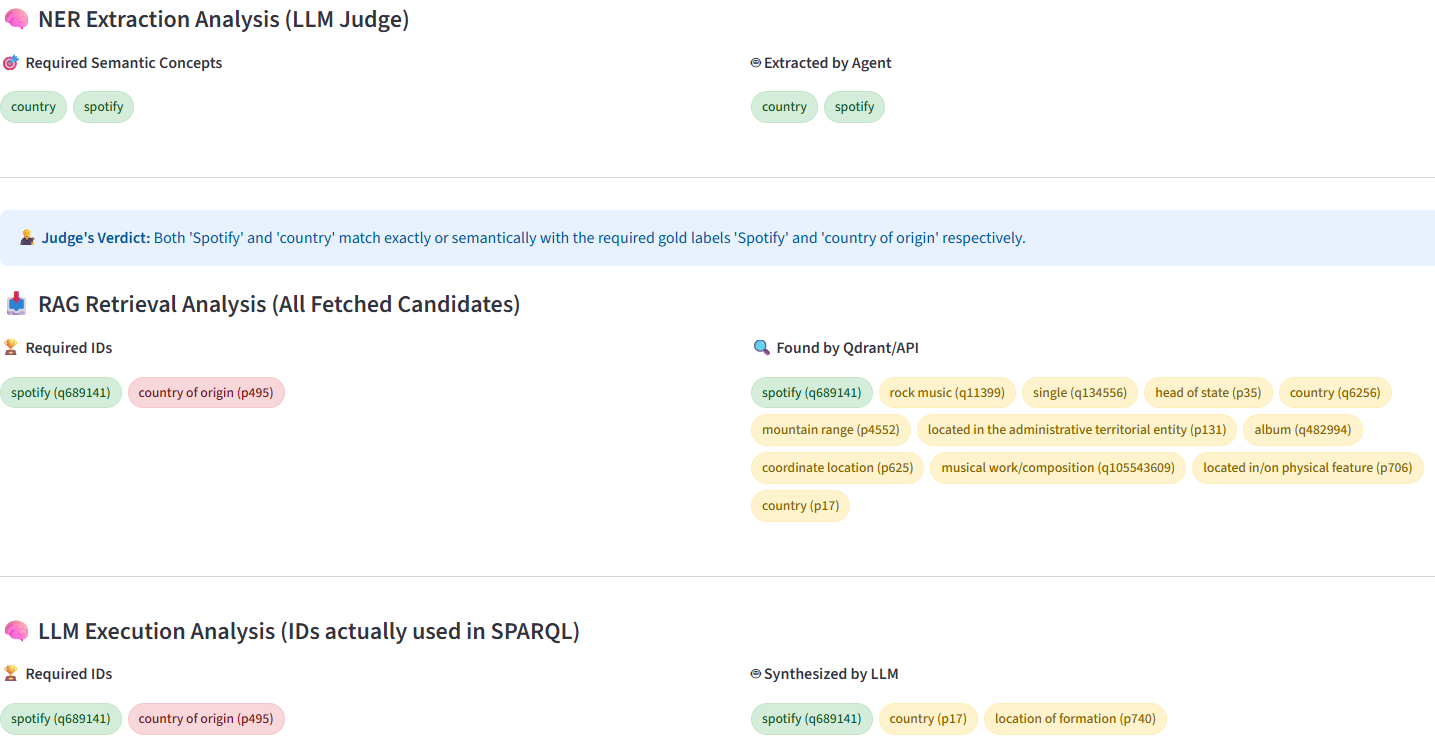
\includegraphics[width=1\textwidth]{Miscellaneous/failure_1.png} 
    \caption{Diagnostic view showing a partial retrieval failure for the question \textit{"In which country was Spotify created?"}. The agent perfectly understood the user's intent (NER chips), but the embedding model only retrieved the Q-node for Spotify, missing the P-node for 'country of origin' (RAG Recall = 0.5).}
    \label{fig:error_rag_partial}
\end{figure}

As shown in Figure~\ref{fig:error_rag_partial} for the query \textit{"In which country was Spotify created?"}, the \texttt{multilingual-e5-small} embedding model successfully retrieved the entity \texttt{wd:Q689141} (Spotify). However, it failed to project the user's intent into the correct Wikidata property, entirely missing \texttt{wdt:P495} (country of origin) which the gold-standard query expected.

Inspecting the generated SPARQL query in Figure~\ref{fig:error_rag_query} reveals an extraordinary emergent behavior from the LLM. 

\begin{figure}[htbp]
    \centering
    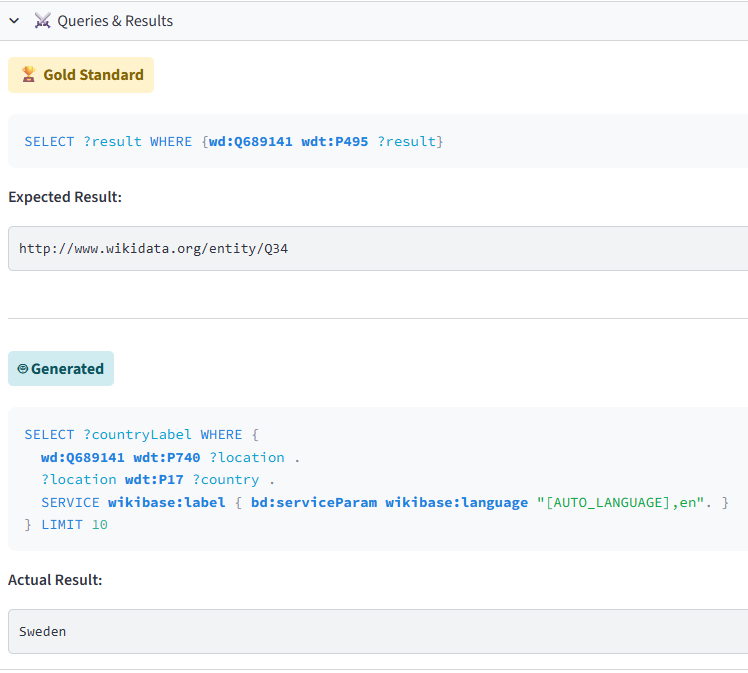
\includegraphics[width=0.95\textwidth]{Miscellaneous/failure_1_query.png} 
    \caption{The LLM's logical workaround. Starved of the direct \texttt{wdt:P495} edge, the agent constructed a 2-hop traversal based on the word "created" to logically deduce the correct factual answer ("Sweden").}
    \label{fig:error_rag_query}
\end{figure}

Because the expected direct property was never injected into its reasoning space, the agent analyzed the subgraph that \textit{was} provided and architected a 2-hop logical workaround. Picking up on the semantic cue of the word "created", it traversed from Spotify using \texttt{wdt:P740} (location of formation) to find the origin city, and then mapped that city to its \texttt{wdt:P17} (country). 

Remarkably, this alternate graph pattern successfully retrieved the factually correct answer ("Sweden"). However, because the QALD-10 benchmark requires the exact 1-hop \texttt{P495} traversal and the raw Wikidata URI, the execution was scored as a 0.0. This example highlights both the vulnerability of dense vector search for specific predicates, as well as the profound reasoning capabilities of foundational agents to logically circumvent database failures when provided with a rich local subgraph.

\subsubsection{Failure Mode 2: NER Collapse and Parametric Recovery (The Variable Binding Penalty)}

The second failure mode highlights a scenario where the initial retrieval pipeline collapses, but the LLM autonomously recovers, only to be penalized by the benchmarking platform's rigid variable naming constraints. This is isolated by filtering for queries with a failing \textit{NER Judge F1} but a perfect mathematical execution.

\begin{figure}[htbp]
    \centering
    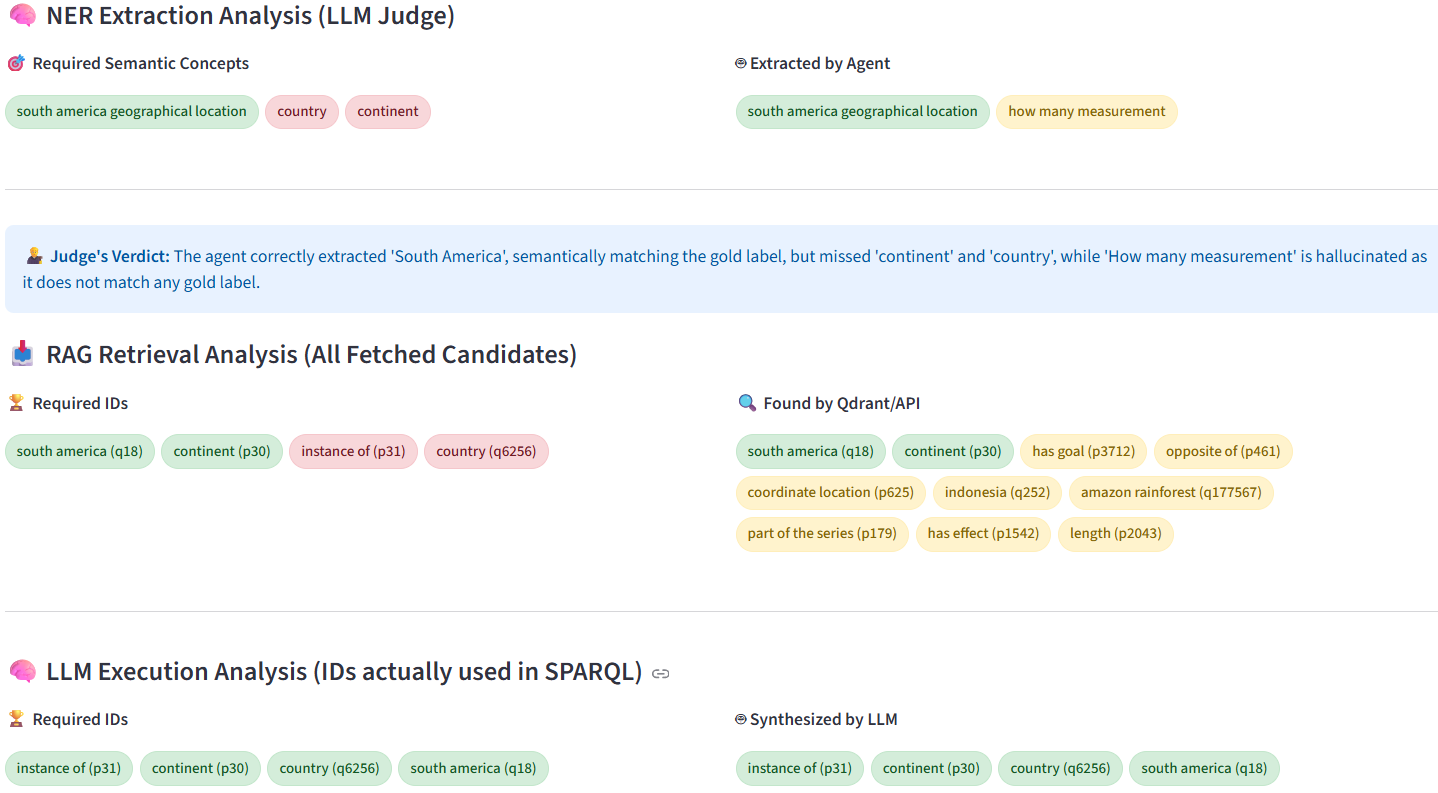
\includegraphics[width=1\textwidth]{Miscellaneous/failure_2.png} 
    \caption{Diagnostic view for the query \textit{"How many countries are on the continent of South America?"}. The NER stage failed to extract "country" (red chip), causing the RAG layer to miss the required ID \texttt{wd:Q6256}. Remarkably, the LLM still synthesized the correct IDs from its parametric memory.}
    \label{fig:error_ner_recovery}
\end{figure}

As shown in Figure~\ref{fig:error_ner_recovery}, the system initially stumbled during the semantic extraction phase. The NER agent identified "South America", but completely missed the required concepts for "country", hallucinating the broad phrase "how many measurement". Consequently, the RAG retrieval layer failed to fetch the required Q-node for country (\texttt{wd:Q6256}) and the structural property for instance of (\texttt{wdt:P31}).

Despite being starved of this critical structural context, the \textit{LLM Execution Analysis} demonstrates a remarkable autonomous recovery. Recognizing that the retrieved context was incomplete, the LLM relied on its pre-trained parametric memory to independently inject \texttt{wdt:P31 wd:Q6256} into the query.

\begin{figure}[htbp]
    \centering
    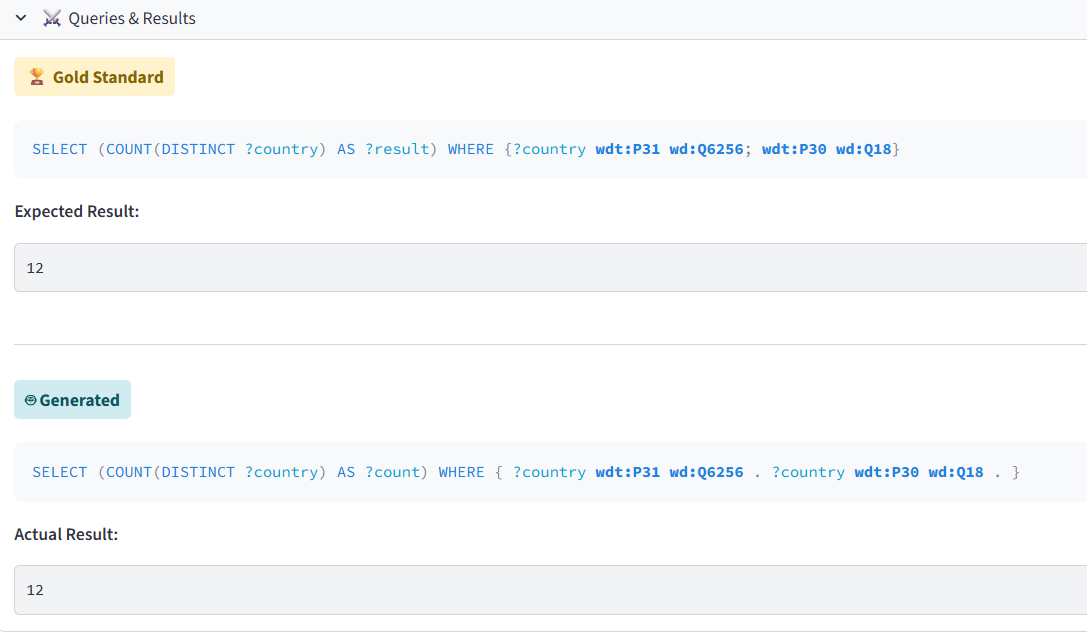
\includegraphics[width=1\textwidth]{Miscellaneous/failure_2_query.png} 
    \caption{The query execution. The LLM successfully constructed the correct logic and retrieved the correct answer ("12"). However, it used \texttt{AS ?count} instead of \texttt{AS ?result}, resulting in a benchmark failure.}
    \label{fig:error_ner_query}
\end{figure}

As illustrated in Figure~\ref{fig:error_ner_query}, the agent's synthesized SPARQL query is logically flawless. It executes successfully against the Wikidata endpoint and returns the exact expected factual answer: \texttt{12}. 

However, this execution was scored as a total failure (0.0 F1) by the GERBIL platform. The QALD-10 benchmark rigidly maps evaluation bindings to specific variable names—in this case, expecting the aggregation to be projected as \texttt{AS ?result}. Because the LLM logically projected the variable as \texttt{AS ?count}, the automated evaluator failed to parse the JSON response. This phenomenon exposes a critical flaw in standardized KGQA benchmarking: systems are frequently penalized for trivial syntactic formatting variances, artificially deflating the reported accuracy of highly capable reasoning agents.

\subsubsection{Failure Mode 3: The Label vs. URI Penalty}

The most nuanced failure mode occurs when the pipeline operates flawlessly—extracting the correct intent and synthesizing valid SPARQL syntax—but is penalized by the rigid exact-match evaluation criteria of the benchmarking platform itself. By filtering for queries where the \textit{NER Judge}, \textit{RAG Recall}, and \textit{LLM Precision} are perfectly maximized (1.0), but the \textit{Final F1 Score} is 0.0, we isolate these boundary cases.

\begin{figure}[htbp]
    \centering
    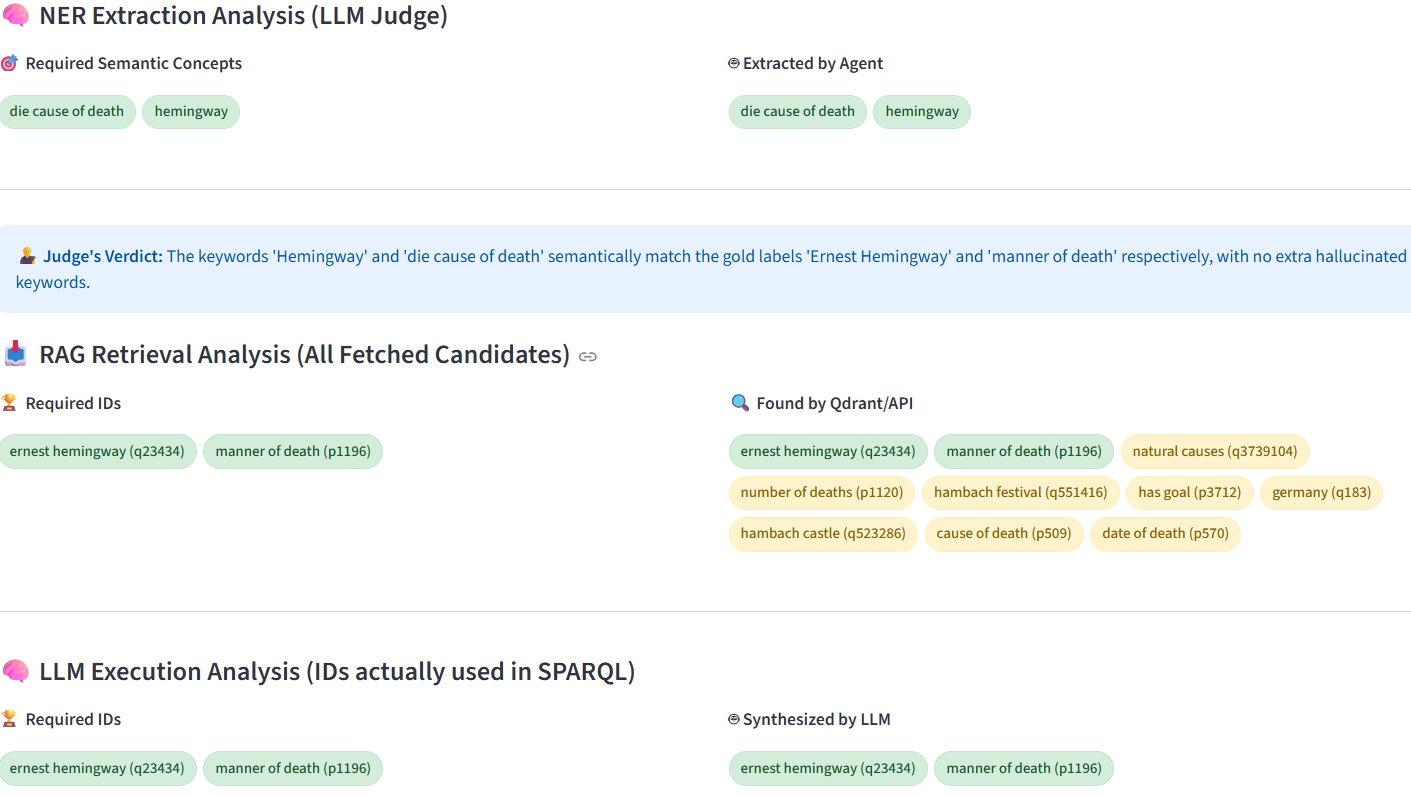
\includegraphics[width=0.95\textwidth]{Miscellaneous/failure_3.png} 
    \caption{Interactive Dashboard highlighting perfect component execution for the question: \textit{"In which manner did Hemingway die?"}. The agent successfully understood the intent, retrieved the correct IDs, and utilized them (all green chips).}
    \label{fig:error_syntax_chips}
\end{figure}

As illustrated in Figure~\ref{fig:error_syntax_chips}, the system's diagnostic trace for the question \textit{"In which manner did Hemingway die?"} demonstrates perfect component execution. The LLM-as-a-Judge verifies that the agent successfully mapped the informal phrasing to the required gold labels. Consequently, the RAG layer retrieved the exact required canonical IDs (\texttt{wd:Q23434} and \texttt{wdt:P1196}), and the LLM explicitly synthesized them into its generated query.

Despite possessing the perfect vocabulary and writing a syntactically valid query, the final execution failed (Final F1 = 0.0). Inspecting the generated SPARQL query reveals the cause of this failure, as shown in Figure~\ref{fig:error_syntax_query}.

\begin{figure}[htbp]
    \centering

    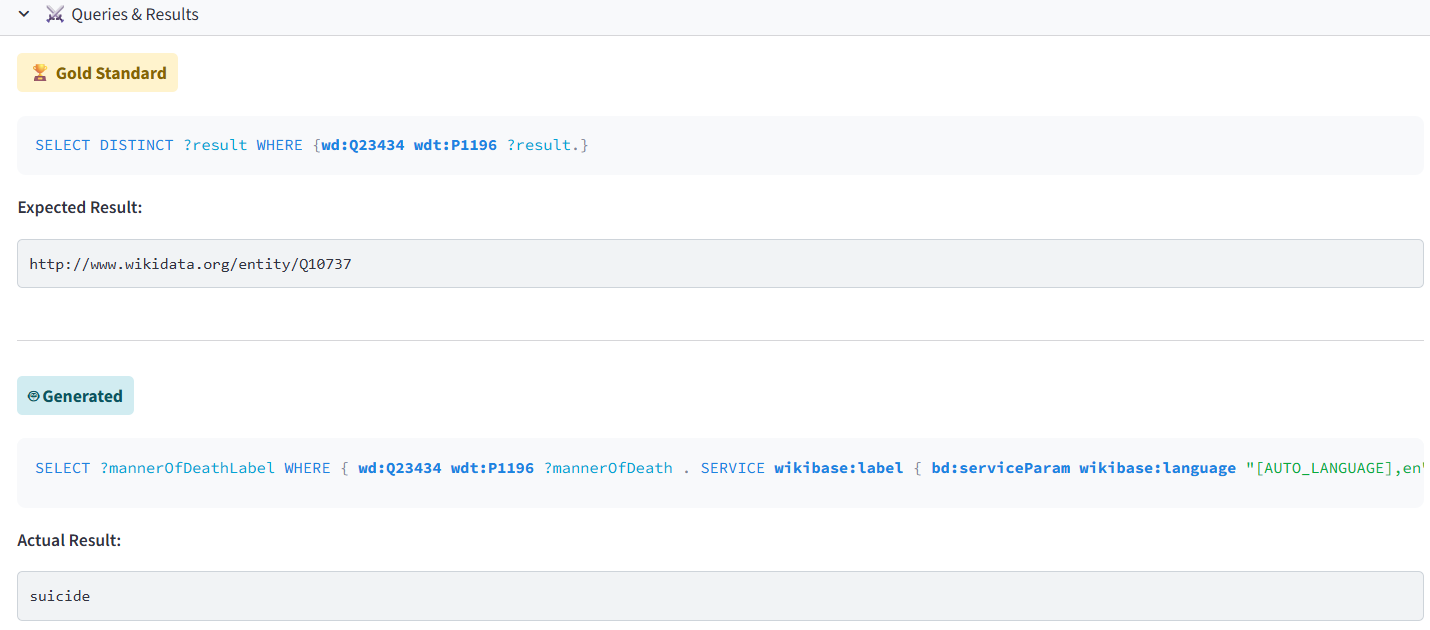
\includegraphics[width=0.95\textwidth]{Miscellaneous/failure_3_query.png} 
    \caption{Comparison of the Gold Standard query and the Generated query. The agent returned the human-readable label ("suicide") instead of the raw Wikidata URI expected by the benchmark.}
    \label{fig:error_syntax_query}
\end{figure}

Because foundational LLMs are instruction-tuned to be helpful to human users, the agent autonomously injected the \texttt{SERVICE wikibase:label} clause. It specifically requested the variable \texttt{?mannerOfDeathLabel}, returning the literal string \texttt{"suicide"}. However, the QALD-10 gold standard evaluates accuracy based on strict URI matching, expecting the raw identifier \texttt{http://www.wikidata.org/entity/Q10737}. 

Because the strict GERBIL evaluation script performs a literal string comparison on the result bindings, it scores this query as a 0.0, despite the agent retrieving the semantically correct answer. This failure mode highlights a critical discrepancy between "benchmark correctness" and "user-facing correctness" in modern Agentic KGQA systems. While the system successfully bridged the natural language gap, navigating rigid benchmark formats requires forcing the LLM to suppress its conversational training and output raw database identifiers.